% !TeX root =thesis.tex

\chapter{Introduction}
Feshbach resonance is widely used in the ultracold alkali gas experiments as a way to tune interaction strength.  This unique ability gives physicists the rare opportunity to study the evolution of many-body system under change of interaction strength, which connects different physics originally developed separately.  Particularly for the fermion system, there was long theoretically work about uniform treatment over BEC and BCS \cite{Eagle,LeggettCrossover,Nozieres,RanderiaBEC}, and Feshbach resonance within the ultracold alkali gas provide the perfect grounds to verify it.  Within the lowest order, the theory works quite well, the experiments fit it qualitatively.  

Here we actually try to look into the idiosyncratic of the Feshbach resonance contrast to a real ``Simple'' knob on the interaction strength.  Within the two-body description of Feshbach resonance, there is a parameter $\delta_c$ describing how close to resonance is necessary to have substantial weight in close-channel.  Moving to a many-body problem, a simple question is how this energy scale compares to a typical many-body energy scale, Fermi energy.  If Fermi energy is much smaller comparing to $\delta_c$, (\emph{broad resonance}), close-channel can be safely ignored at many-body level and the problem can be well-described as a two-species fermion system with tunable interaction.  On the contrary, when Fermi energy is larger than or comparable to $\delta_c$, close-channel cannot be ignored in many-body level.  Nevertheless, another important thing in the problem is that we are dealing with a Feshbach resonance with a relatively tight-bound close-channel state, which is much smaller comparing to other many-body scale, such as inter-particle distance, (but often larger than potential range though).  Therefore, we are never dealing with a true three(four)-species Fermion system, which probably requires quite different techniques to solve.

To complicate the problem even further, the real experiments system often has one common species between two channels.  Pauli exclusion prevents the same species occupy both channels.  This effect has no counter-part in two-body physics, and is one of the central problems in this study. 

Roughly speaking, many-body nature brings three effects.  The first one closely associates with Fermi energy.  At low temperature, most fermions are inactive and only fermions close to fermi surface can participate, therefore, energy often needs to be measured from Fermi sea instead of zero as in two-body situation.  It always relates to Fermi Energy $E_F$.    We mostly dealing with This effect has been extensively studied in \cite{GurarieNarrow}.

Unlike single-channel problem, there are two densities for two channels. When close-channel weight is small (broad resonance), it is all right to treat the total density as the same of open-channel density.  However, in the narrow resonance, where close-channel weight is not negligible, the counting needs to be careful.  This effect is also extensively studied in \cite{GurarieNarrow}.

The last effect is unique for the three-species problem, where one common species show in both channels.  Phase spaces of two channels are overlapped because of the Pauli exclusion from the common species. This effect is controlled by overlapping of states in two channels. We can estimate it roughly.  In the close-channel, bound-state is relatively small, and binding energy $E_b$ is close to absolute energy difference between two channels, $\eta$, around resonance.  On the other hand, fermions in open-channel occupies the lowest states in the momentum space and therefore spread out in space.  The typical energy scale would be $E_F$.  Therefore a ratio $E_F/\eta$ would control such effect. How such factor affect the system is the center of this thesis. 

Alternatively, we can make a rough estimation on simple double-fermion molecule gas.  If we assume the molecule size is $r_{c}$ and the total number is $N$.  If assume further that the bound-state is close-to-threshold.  We will have wave function $A/(k^{2}+\kappa^{2})$, where $\hbar^{2}\kappa^{2}/2m=E_{b}$, (see Appendix \ref{sec:pathInt2:short-range}) and $\sum_{k=0}^{1/r_{c}}\psi^{2}\sim{}N$, now if we considering only particles within range $E_{F}\ll\kappa$, the total particle in it is roughly $N\cdot(k_{F}r_{c})$.  this number can be much smaller than $N$. Put this into the perspective of two-channel problem, the low-momentum is still dominated by open-channel component even when total weight of close-channel is comparable or higher than it of open-channel because close-channel is mostly in high-momentum state, and in the low-momentum, open-channel still dominates.     

We will introduce several concepts important to our study in the following sections and study the narrow resonance problems in detail in Chapter \ref{ch:path2}. And we will discuss and conclude our approach in Chapter \ref{ch:conclusion}.

\section{Dilute ultracold Alkali gas}
\subsection{Hyperfine species}
TO BE COMPLETED. 


\section{S-wave scattering length, Bethe-Peierls boundary condition, universality, two-body density matrix\label{sec:intro:as}}
In dilute ultracold Alkali gas, both the density and temperature are so low that in most case, the interaction can be characterized by a single two-body parameter, s-wave scattering length, $a_s$.  Most case this is  interpreted as we can replace the real potential as a pseudo potential\cite{pethick}.  Nevertheless, an alternative interpretation about $a_s$ is more useful in this work\cite{LeggettBEC, Tan2008-1,Tan2008-2,CombescotTan}.  For short-range potential, where potential range $a_c$ is much smaller than average inter-particle distance $a_0$, it is not hard to see in the majority of the space, $\mathcal{D}$, particles are free-like, they only interact when close to each other, $\mathcal{I}$.  In the very dilute case, most physical quantities can be calculated only considering the free part, $\mathcal{D}$.  The effect of the potential and short-range wave-function, $\mathcal{I}$, is to enforce the boundary condition on free part $\mathcal{D}$, 
\begin{equation}\label{eq:intro:Bethe}
\psi(r)\xrightarrow{r\to0}\nth{r}-\nth{a_s}
\end{equation}
which is also known as Bethe-Peierls boundary condition\cite{BethePeierls}.  This boundary condition applies to two-body, few-body, as well as many-body physics.  

In two-body physics, note we did not mention anything about zero energy, where $a_{s}$ is defined in scattering theory context, and indeed this boundary condition applies generally to  any weak (positive or negative) energy solution as long as the energy involved is much lower than the energy scale in internal region $\mathcal{I}$.  Therefore it is easy to extend it to close-to-threshold bound state.  A weak bound-state has wave function $\psi(r)=\nth{r}e^{-r/a_s}$ in $\mathcal{D}$,\footnote{The extra $\nth{r}$ factor is there for  radial wave function in 3D.} which matches Bethe-Peierls boundary condition with a positive $a_{s}$ (for  $r\ll{}a_{s}$), and we have the often cited relation for binding energy $E_{b}$.
\begin{equation}
 E_{b}=\frac{\hbar^{2}}{2ma_{s}^{2}}
\end{equation}
  This immediately explains one often confusing and counter-intuitive fact, that positive  $a_s$ corresponds to bound state.  If interpreting in the normal scattering theory, positive $a_s$  usually associates with the repulsive interaction, which obviously does not support a bound state.\footnote{This seemingly paradox can be resolved carefully within scattering theory as following. In scattering theory, the fact,  repulsive interaction leads to positive phase shift and therefore positive $a_s$, and attractive interaction leads to negative phase shift and negative $a_s$, is only true when interaction is weak, phase shift and $a_s$ is small.  At the strong interaction, where bound state is formed, phase shift changes $\pi$; $a_s$ is large and  change sign over the threshold. }

 S-wave scattering length, $a_s$, or Eq. \ref{eq:intro:Bethe}, does not fix the normalization on the wave function. This normalization factor, turns out to be very useful.  Its square is just \emph{integrated contact intensity}, $C$, \cite{ Tan2008-1,Tan2008-2,CombescotTan}, besides a simple constant factor.  At the limit where $a_c\to0$, $C$ and $a_s$ alone, can describe several important physical quantities, (for example internal energy).  A particular useful one for this thesis is the limit at high-momentum distribution of particles, 
 \begin{equation}
 n_k=\frac{C}{k^4}
 \end{equation}
 Note that here actually high-momentum means lower than the characteristic momentum of potential $1/a_c$, but higher than any other scale, $1/a_0$,...
 
 In many-body, lots of physical observable quantities relate to one set of  quantities, density matrix, $\av{\Psi^\dg\Psi^\dg\cdots\Psi\Psi}$. In fermionic system,  one-body density matrix is often very close to the free case and not very interesting, especially when we are interested in properties involving fermion pairs.  Two-body density matrix is often used. Formally, we can decompose it into orthogonal basis
 \begin{equation}
 \av{\Psi^\dg(x_1)\Psi^\dg(x_2)\Psi(y_2)\Psi(y_1)}=\sum_nC_n\phi_n^\dg(x_1,x_2)\phi_n(y_1,y_2)
 \end{equation}     
 When one or a few $C_n$ is macroscopic, the system behaves quantum mechanically in macroscopic term.  Especially when only one term is macroscopic, system can often be interpreted as one macroscopic wave function.\cite{Leggett}  This can serves as the starting point for several phenomenon, such as BEC, BCS superconductor,...
 
Shizhong and Leggett developed independently another universality theory based on two-body density matrix \linebreak[2] \cite{shizhongUniv}, which actually takes a more general case.   They asserted that for short-range potential and low temperature, for example dilute ultracold alkali gas, the basis wave functions $\phi_n$ follows the two-body wave function at short-range. This is actually similar as Bethe-Peierls boundary condition Eq. \ref{eq:intro:Bethe}.  And not surprisingly, many physical properties are determined by the normalization factors.  

In this thesis, similar idea is used along this line.  However, open-channel does not follow its two-body short-range wave-function because sensitive nature of resonance. 
 
 
 \section{Two-body Feshbach resonance\label{sec:intro:twobody}}
Here we will briefly review the Feshbach resonance in two-body system.   As discussed in the previous section, for isolated single atom, hyperfine level is the eigenstate.  However, when two atoms interacts, most of interaction comes from interaction of electrons while nucleons interacts very little.  Therefore, hyperfine levels is no longer true eigenstates of the two-body system and two hyperfine.  Nevertheless, hyperfine level serves a good approximated quantum number and levels are still labelled with it. Furthermore, we take ``channels'' as pair of hyperfine indices, they are in general different in interaction strength and are decoupled in the lowest order.  In magnetic field, different channels differ in energy mostly due to the Zeeman energy of electronic spin as electronic magnetic moment is much larger than nuclear magnetic moment.  This energy difference is easy to tune via magnetic field.  

When mixture between channels are taken into consideration, the simple single-channel scattering becomes multi-channel scattering.  Especially, when the one channel's threshold is close to a bound-state in the other channel when considered isolated, the scattering property in this channel is dramatically altered,  phase shift can changes $2\pi$ and s-wave scattering length $a_{s}$ changes to infinity and jumps to the infinity in opposite sign.  This is essentially what happens in Feshbach resonance, which was studied by Fano\cite{Fano} and Feshbach \cite{nuclear}  in nuclear and atom physics 1960s.  Here we will mostly follow treatment in \cite{Leggett} (with some different symbols to confirm with the rest of this thesis). 
\footnote{Here I list a few main different symbols, with the symbols from \cite{Leggett} in parenthesis.  $U$ ($=-V$): open-channel interaction; $V$ ($=-V_{c}$): close-channel interaction; $Y$ (=-$g\cdot{}f$): inter-channel coupling; $E_{b}$ ($=\epsilon_{0}$):binding energy of close-channel bound state; $a_{c}$ ($=r_{0}$): range of potential; $\eta$ ($=\epsilon_0+\tilde\delta$) the Zeeman energy difference between two channels; $\mathcal{K}$ ($=\kappa$) see Eq.\ref{eq:intro:kappa}.}

Here we schematically call two channels as $\ket{\uparrow}$ and $\ket{\downarrow}$.  And the hamiltonian in this ``spinor'' space is (assumed isotropic)
\begin{equation}
\hat{H}(r)=
\begin{pmatrix}
-\frac{\hbar^{2}}{2m_{r}}\nabla^{2}-U(r)&-Y(r)\\
-\frac{\hbar^{2}}{2m_{r}}\nabla^{2}+\eta-V(r)&-Y(r)
\end{pmatrix}
\end{equation}
Here we count energy zero from that of the open channel at infinite separation, $\eta$ is the absolute difference in Zeeman energy of two channels.  And all the interactions are short-range.  For a s-wave solution we have 
\begin{equation}
\psi(r)=\nth{r}\bbr{\chi(r)\ket{\uparrow}+\chi_{c}(r)\ket{\downarrow}}
\end{equation}
Now we can write down the time-independent \sch equation in radial direction for the scattering state:
\begin{align}
-\frac{\hbar^{2}}{2m_{r}}\chi''-U\chi-Y\chi_c&=E\chi\label{eq:intro:open}\\
-\frac{\hbar^{2}}{2m_{r}}\chi_c''+\eta\chi_c-V\chi_c-Y\chi&=E\chi_c
\end{align}
Here we expand $\chi_{c}$ over the eigenstates of close-channel hamiltonian, $\phi_{i}$, 
\begin{equation}
-\frac{\hbar^{2}}{2m_{r}}\phi_{i}''-V \phi_{i}=-E_{b}^{(i)}\phi_{i}
\end{equation}
Here we assume the energy difference between levels are larger than other energy scale and keeps only the one in resonance, $\phi_{0}$.  Na\"{i}vely speaking, the resonance happens at the point where the close-channel bound state level is exactly at the threshold of open-chanel.  Therefore we introduce the relative detuning, $\tilde\delta=\eta-E_{b}$ It is not hard to find
\begin{equation}
\chi_{c}=\frac{\phi_{0}}{E-\tilde\delta}\int{dr'}\,\phi_{0}^{*}(r')Y(r')\chi_{r'}
\end{equation}
Note that here $\phi_{0}$ is normalized (for radial component).  Put this back to \sch equation of open-channel component $\chi$ (Eq. \ref{eq:intro:open}), 
\begin{equation}\label{eq:intro:chi}
\br{-\frac{\hbar^{2}}{2m_{r}}\frac{d^{2}}{dr^{2}}-U-E}\chi+\frac{1}{E-\tilde\delta}\int_{0}^{\infty}K(r\,r')\chi(r')dr'=0
\end{equation}
where kernel $K(r\,r')$ is
\begin{equation}
K(r\,r')\equiv\phi_{0}(r)\phi_{0}(r')Y(r')Y(r)\equiv{}K(r'\,r)
\end{equation}
Compare this with open-channel scattering \sch equation without coupling to close-channel
\begin{equation}\label{eq:sec:chi0}
\br{-\frac{\hbar^{2}}{2m_{r}}\frac{d^{2}}{dr^{2}}-U-E}\chi_{0}=0
\end{equation}
Note that $\chi_{0}(r)\rightarrow0$ as $r\rightarrow0$ and $\chi_{0}(r)\rightarrow\text{const}(1-r/a_{bg})$ for $r\rightarrow\infty$\footnote{Note that we are dealing with the internal wave function $\chi_{0}$ here instead of the external wave function as in Sec. \ref{sec:intro:as}, therefore, the boundary condition for $r\rightarrow0$ there actually corresponds boundary condition $r\rightarrow\infty$ here.}  Now multiply Eq. \ref{eq:intro:chi} with $\chi_{0}$ and Eq. \ref{eq:intro:chi0} with $\chi$, subtract them, and use Green's theorem, we find 
\begin{equation}
\chi_{0}(r_{c})\chi'(r_{c})-\chi_{0}'(r_{c})\chi(r_{c})+\frac{2m_{r}E}{\hbar^{2}}\int_{0}^{r_{c}}dr\chi_{0}(r)\chi(r)
=\frac{2m_{r}/\hbar^{2}}{E-\tilde\delta}\int_{0}^{r_{c}}dr\int_{0}^{r_{c}}dr'\chi_{0}(r)K(rr')\chi(r')
\end{equation}
Here $r_{c}$ is a large distance, and we can use the boundary condition by let $r\rightarrow\infty$, $\chi_{0}(r)\rightarrow\text{const}(1-r/a_{bg})$, $\chi(r)\rightarrow\text{const}(1-r/a_{s})$.  The R.H.S approaches a constant for a short-range interaction $Y(r)$ and therefore $K(rr')$.  For scattering solution at  $E=0$, we have 
\begin{equation}
\nth{a_{s}}-\nth{a_{bg}}=\frac{2m_{r}/\hbar^{2}}{\tilde\delta}\int_{0}^{\infty}dr\int_{0}^{\infty}dr'\chi_{0}(r)K(rr')\chi(r')
\end{equation}
It is easy to see that contrary to na\"ive intuition, $a_{s}$ does not diverge at the point $\tilde\delta=0$ because of the original interaction in open-channel, $a_{bg}$.  We can define a quantity $\mathcal{K}$, as the detuning where $a_{s}$ diverges, by the implicit equation ($\mathcal{K}$ shows up in R.H.S as well)
\begin{equation}\label{eq:intro:kappa}
\mathcal{K}\equiv-\frac{2m_{r}a_{bg}}{\hbar^{2}}\int_{0}^{\infty}{dr}\int_{0}^{\infty}dr'\chi_{0}(r)K(rr')\chi_{\tilde\delta=\mathcal{K}}(r')
\end{equation}
And if we define the ``real detuning'' $\delta\equiv\tilde\delta-\mathcal{K}$, we have 
\begin{equation}
a_{s}(\delta)=a_{bg}\br{1+\frac{\kappa}{\delta}}
\end{equation}
Comparing this with the empirical formula of Feshbach resonance
\begin{equation}
a_{s}(B)=a_{bg}\br{1+\frac{\Delta{B}}{B-B_{0}}}
\end{equation}
We see that $\Delta{B}=\mathcal{K}(\partial\delta/\partial{B})^{-1}$, and $B_{0}$ is the real resonance position.  Here $\partial\delta/\partial{B}$ is the magnetic momentum difference between two channels.  

Next we consider the bound state where $E<0$, define
\begin{equation}
a_{b}(E)\equiv\frac{\hbar}{(2m_{r}\abs{E})^{1/2}}
\end{equation}
Note that $a_{b}(E)$ is not identified as $a_{s}$ a priori.  Here we only study the bound state close to threshold with binding energy much smaller than the binding energy of close-channel bound state $\phi_{0}$, $\abs{E}\ll\epsilon_{0}$.  Outside the range of potential $a_{c}$,  Going through the similar procedure as previous, the 









As we discussed in Sec. \ref{sec:intro:as}, two-particle interaction is often approximated by a pseudo-potential characterized with s-wave scattering length $a_{s}$ in a dilute system.   The drastic  change  of $a_{s}$  via tuning energy difference (magnetic field)between two channels in Feshbach resonance gives the rare ability to experimentalists to varying the interaction strength between two channels.  And it is extremely useful in the study of BEC-BCS crossover which covers the variation of exact this nature.  


\section{Single-channel BEC-BCS crossover}
Here we will briefly review the BEC-BCS crossover in single channel.   Here the interaction strength is tuned along the crossover region.  This applies to the broad-resonance, where the close-channel weight is negligible and serves only to modify the effective strength in open-channel.  We will mostly follow treatment in \cite{RanderiaBEC, Randeria1997, Randeria2008}.
%\subsection{Path integral for one channels}
% !TeX root =thesis.tex
%\subsection{Path integral approach for single channel\label{sec:pathInt}}
\label{sec:pathInt}
They have studied this problem with a path integral approach which is proved to be a  nice tool for the problem due to its flexibility and readiness to be   extended for the higher order fluctuations.  In the next two chapters, this method will be adapted  further for the two-channel model. 

We start with an attractive $\delta$-potential in the coordinate space.  This potential is not equivalent to the  reduced pairing potential used in the original BCS work.  The reduced pairing potential only couples  particles of the opposite momentum and does not support simple form of Hubbard-Stratonovich transformation, which is essential to solve the problem in the path integral formulation. 

  The Hamiltonian with the chemical potential of the system can be written as   
\begin{equation}
\hat{H}-\mu\hat{N}=\sum_{\sigma}\int{d^{d}\vr}c^{\dagger}_{\sigma}(\vr)\br{-\nth{2m}\nabla^{2}-\mu}c^{}_{\sigma}(\vr)-g\int{d^{d}\vr}c^{\dagger}_{\uparrow}(\vr)c^{\dagger}_{\downarrow}(\vr)c^{}_{\downarrow}(\vr)c^{}_{\uparrow}(\vr)
\end{equation}
Introducing the quantum partition function $\mathcal{Z}=\int{\bigD(\bar\psi,\psi)\exp\br{-S[\bar\psi,\psi]}}$, where $\bigD(\bar\psi,\psi)$ denotes the functional integral over all possible wave function $\psi$ and $\bar\psi$, and the action $S[\bar\psi,\psi]$ can be written down from the Hamiltonian
\begin{equation}\label{eq:pathInt2:actionPsi}
S[\bar\psi,\psi]=\int^{\beta}_{0}d\tau\int{d^{d}\vr}\mbr{\sum_{\sigma}\bar\psi_{\sigma}(\vr,\tau)\br{\partial_{\tau}-\nth{2m}\nabla^{2}-\mu}\psi_{\sigma}(\vr,\tau)-g\bar\psi_{\uparrow}(\vr,\tau)\bar\psi_{\downarrow}(\vr,\tau)\psi^{}_{\downarrow}(\vr,\tau)\psi^{}_{\uparrow}(\vr,\tau)}
\end{equation}
The fermion fields $\psi_{\sigma}$ and $\bar\psi_{\sigma}$ being two independent Grassmann variables, notice that  they are not complex conjugate to each other as in the usual operator language because  complex conjugate is not a well-defined concept for Grassmann variables. 

This system can be solved with Hubbard-Stratonovich transformation.   Introduce an auxiliary field (functional variable) $\Delta(\vr,\tau)$ coupled with a pair $\psi_{\uparrow}(\vr,\tau)\psi_{\downarrow}(\vr,\tau)$. %Here we follow the normal notation from path integral, $r$ is four tempo-space coordinator.  
We write down first the Gaussian integral of $\Delta$
\begin{equation}
1=\int{\bigD(\bar\Delta,\Delta)}\exp\br{-\nth{g}\int{d\tau{d}^{d}r}\bar\Delta\Delta}
\end{equation}
Note that we absorb the extra constant of integration into the measure of $\bigD(\bar\Delta,\Delta)$.
And with a shift of $\Delta(\vr,\tau)\rightarrow\Delta(\vr,\tau)-g\psi_{\uparrow}(\vr,\tau)\psi_{\downarrow}(\vr,\tau))$, we have 
\footnote{$\int{\bigD(\bar\Delta,\Delta)}\cdot1$ is only a constant factor on partition function $\mathcal{Z}$ and has no effect on real physical quantity; therefore, we can take it as 1. (This is equivalent to  divide the $\mathcal{Z}$ by a constant)}
\begin{equation}\label{eq:pathInt:expHS}
\exp\br{g\int{d\tau{}d^{d}r}\bar{\psi}_{\uparrow}\bar\psi_{\downarrow}\psi_{\downarrow}\psi_{\uparrow}}=
\int{\bigD(\bar\Delta,\Delta)}\exp\bbr{-\int{d\tau{d^{d}r}}\mbr{\nth{g}{\bar\Delta}{\Delta}-\br{\bar\Delta\psi_{\downarrow}\psi_{\uparrow}+\Delta\bar\psi_{\uparrow}\bar\psi_{\downarrow}}}}
\end{equation}
Note that  $\Delta(\vr,\tau)$ (or $\bar\Delta(\vr,\tau)$) comes from  Grassmann fields $\psi(\vr,\tau)$ (or $\bar\psi(\vr,\tau)$). Therefore, they are not related to each other as complex conjugate either.  Nevertheless, at the mean field level or only at the phase fluctuation around the mean field values, $\Delta$  and $\bar\Delta$ are indeed complex conjugate.  Consequently, we will just take $\Delta$  as normal bosonic field in the following and often simply treat $\bar\Delta$ as $\Delta$'s complex conjugate in the following. Now the interaction term can be replaced.
\begin{align*}
\mathcal{Z}=&\int{}\bigD(\bar\psi,\psi)\int{\bigD(\bar\Delta,\Delta)}\\
&\;\exp\bbr{-\int{d\tau{d^{d}r}}\mbr{\sum_{\sigma}\bar\psi_{\sigma}\br{\partial_{\tau}-\nth{2m}\nabla^{2}-\mu}\psi_{\sigma}+\nth{g}{\bar\Delta}{\Delta}-\br{\bar\Delta\psi_{\downarrow}\psi_{\uparrow}+\Delta\bar\psi_{\uparrow}\bar\psi_{\downarrow}}}}
\end{align*}
At the expense of introducing an auxiliary field ($\Delta$) which has contact-type coupling to the original field $\psi$, we eliminate the four-field interaction term formally.  $\Delta$ field is like a \emph{local potential} for $\psi$, although this \emph{local potential} has to be calculated from the original field self-consistently.  Nevertheless, $\Delta$ couples to a pair of fermionic field $\psi$, and thus it extracts a special degree of freedom from the $\psi$ field.  When properly selected, this degree of freedom is highly non-trivial and has macroscopic importance, which serves as ``order parameter'' for the system.  The above formula for partition function is bilinear to $\psi$, and we can rewrite it into a nicer form in Nambu spinor representation
\begin{equation}
\bar\Psi=\begin{pmatrix}\bar{\psi}_{\uparrow}&\psi_{\downarrow}\end{pmatrix}\text{,  }\qquad
\Psi=\begin{pmatrix}{\psi}_{\uparrow}\\\bar\psi_{\downarrow}\end{pmatrix}
\end{equation}
\begin{equation}\label{eq:pathInt:ZDeltaPhi}
\mathcal{Z}=\int{\bigD(\bar\Psi,\Psi)}\int{\bigD(\bar\Delta,\Delta)}\exp
	\bbr{-\int{d\tau{d^{d}r}}\mbr{\nth{g}{\bar\Delta}{\Delta}-\bar\Psi \nG\Psi}}
\end{equation}
where 
\begin{equation}\label{eq:pathInt:nG}
\nG=\begin{pmatrix}
[\hat{G}_{0}^{(p)}]^{-1}&\Delta\\\bar\Delta&[\hat{G}_{0}^{(h)}]^{-1}
\end{pmatrix}
\end{equation}
is known as the Gor'kov Green function. $[\hat{G}_{0}^{(p)}]^{-1}=-\partial_{\tau}+\nth{2m}\nabla^{2}+\mu$, and $[\hat{G}_{0}^{(h)}]^{-1}=-\partial_{\tau}-\nth{2m}\nabla^{2}-\mu$ represent the non-interacting Green functions of the particle and the hole respectively. 

Before going further, we would like to discuss one confusing point about the possible one-or-two indices for quantities such as ${G}$ or $\Delta$ in Eq. \ref{eq:pathInt:nG}.  As a matrix, such a quantity has two indices $(x,x')$ or $(p,p')$, which have no ambiguity in usage. On the other hand, there are often ambiguity when only one index $x$ or $p$ is used. In some cases, the one index means the relative value of the two indices. For example, an  interaction, $U(\vr_{1},\vr_{2})$, normally only depends on the relative coordinate, $\vr=\vr_{1}-\vr_{2}$. So $U(\vr)$ means $U(\vr_{0}+\vr,\vr_{0})$.  In other cases, especially common in the current thesis, the one index stands for its repetition.  In this case, the difference is always zero. For example, the free Green's function, $G_{0}(p)$ stands for $G_{0}(p,p')\delta({p-p'})$.  Similarly,  the order parameter, $\Delta(x)$, only couples to $\bar\psi(x)\bar\psi(x)$ (Eq. \ref{eq:pathInt:expHS}).  When used in the matrix context (Eq. \ref{eq:pathInt:nG}), it means $\Delta(x)\delta(x-x')$. Interestingly, its Fourier transformation in momentum space does not have the same properties.  In fact, it means $\Delta(p,p')=\Delta(p'-p)$.

Now action in Eq. \ref{eq:pathInt:ZDeltaPhi} is bilinear to $\Psi$; so it can be integrated out formally and the partition function then only depends on the  field $\Delta$.  
\begin{equation}\label{eq:pathInt:DeltaPF}
\mathcal{Z}=\int{\bigD(\bar\Delta,\Delta)}\exp
	\bbr{-\mbr{\br{\int{d\tau{d^{d}r}}\nth{g}{\bar\Delta\Delta}}-\ln\det\nG}}
\end{equation}
And the action becomes
\begin{equation}\label{eq:pathInt:DeltaAction}
S[\bar\Delta,\Delta]=
	{\mbr{\br{\int{d\tau{d^{d}r}}\nth{g}{\bar\Delta\Delta}}-\ln\det\nG}}
\end{equation}
Note that the determinant in $\ln\det\nG$ runs through both the normal coordinate space and $2\times2$ Nambu spinor space.  The above formulas are exactly equivalent to the original partition function (action) in the fermion field $\psi$ (Eq. \ref{eq:pathInt2:actionPsi}). It looks nice and compact. Nevertheless, $\ln\det\nG$ term is highly non-trivial and contains all the many-body physics.

\section{Mean field results\label{sec:pathInt:meanfield}}
The saddle point equation of Eq. (\ref{eq:pathInt:DeltaPF}) gives the mean-field result of the system.  First we need to find the derivative of $\ln\det\nG$.  We notice the identity
\begin{equation}
\ln\det\hat{A}=\tr\ln\hat{A}
\end{equation}
and differential rule of the function ``$\tr\ln$''
\begin{equation}\label{eq:pathInt:diffTr}
\frac{\delta}{\delta\phi_q}\tr\ln(\nG)=\tr(\hat{\mathcal{G}}\frac{\delta}{\delta\phi_q}\nG)
\end{equation}
Using the above relations, we can write the saddle equation of Eq. (\ref{eq:pathInt:DeltaPF}) (differential with respect to $\Delta$) as
\begin{equation}
\nth{g}\bar{\Delta}(\vr,\tau)-\tr\mbr{\hat{\mathcal{G}}(\vr,\tau,\vr,\tau)\begin{pmatrix}0&1\\0&0\end{pmatrix}}=0
\end{equation}
Here this matrix is in the Nambu Spinor space.  At the  mean field level, we seek a tempo-spacial homogeneous solution of $\Delta(x)=\Delta_{0}$.  At this level,  $\Delta(p)$ becomes a $\delta$-function in the frequency-momentum space, and has non-zero elements only for two fermions with the same momentum.  (Please See the discussion in the previous section about one vs. two indices. This is not generally true, as we show it when discussing collective modes in sec. \ref{sec:collective1})
We can find the Gor'kov Green function from Eq. (\ref{eq:pathInt:nG}) in momentum space at the mean-field level
\begin{equation}\label{eq:pathInt:G0}
G_{0\;p,p'}=\nth{(i\omega_n)^2-E_\vp^2}
\begin{pmatrix}
	i\omega_n+\xi_\vp&\;&-\Delta_0\\
	-\bar{\Delta}_0&\;&i\omega_n-\xi_\vp
\end{pmatrix}
\delta_{p=p'}
\equiv{}G_{0}(p)\delta_{p=p'}
\end{equation}
Here $p$ is the frequency-momentum, $p=(\omega_{n},\vp)$, and $\omega_n$ is the Matsubara frequency of Fermions.  $\xi_{\vk}=\epsilon_{\vk}-\mu$, $\epsilon_{\vk}=\vk^{2}/2m$,  $E_\vp=\sqrt{\xi_\vp^2+\abs{\Delta_0}^2}$.  And the saddle point equation can be rewritten as 
\begin{equation}
\nth{g}\bar{\Delta}_0=\frac{T}{\mathcal{V}_{0}}\sum_{\vp,n}\frac{\bar\Delta_0}{\omega_n^2+E_\vp^2}
\end{equation}
Here $T$ is the temperature, and $\mathcal{V}_{0}$ is the volume in $d$-dimension.  The summation of Matsubara frequency  can be evaluated\footnote{\label{foot:intro:sum}The summation of the Matsubara frequency of a function $h(i\omega_{n})$ is carried out by the normal trick.  We  multiply $h(z)$ with the Fermi distribution function $n_{F}(z)$,  the summation is the sum of residuals at the imaginary axis of $n_{F}(z)$.  The contour can be deform into a contour over the rest of singular points of $h(z)$. We just need to find the residuals of the total function $h(z)n_{F}(z)$ over those singular points to find the Matsubara summation.   However, due to zero temperature, the  $n_{F}(z)$ is only nonzero at the negative singular points of $h(z)$, $-E_{\vk}$ in this case.  (The other singular point $E_{\vk}$ gives $n_{F}(E_{\vk})=0$ for zero temperature.)}  and we find 
\begin{equation}
\nth{g}=\nth{\mathcal{V}_{0}}\sum_{\vp}\frac{1-2n_f(E_p)}{2E_p}=\nth{\mathcal{V}_{0}}\sum_{\vp}\frac{\tanh{(E_p/2T)}}{2E_p}
\label{eq:pathInt:gap}
\end{equation}
where $n_f(\epsilon)$ is the fermi distribution function.  This is exactly the famous gap equation obtained from other methods as well.  On the other hand, $\nG$ in Eq. (\ref{eq:pathInt:nG})  is the inverse of the  fermion-fermion correlation of $\Psi$.  In the mean field, $G_{0}$ as Eq. (\ref{eq:pathInt:G0}) can be diagonalized in the momentum space with a canonical (Bogoliubov) transformation.  We can make an analytic continuation of $i\omega_{n}\rightarrow\omega+0^{+}$.  Eq. (\ref{eq:pathInt:G0})  then has poles ($\pm{}E_{p}$) where  $\omega^2-E_\vp^2=0$,  which determine  the spectrum of fermionic excitation.  Indeed, in the BCS-like states ($\mu>0$), the spectrum is gapped at $\Delta$; while in the BEC-like states ($\mu<0$), the fermionic excitation starts from the molecule binding energy $\sqrt{\mu^{2}+\Delta^{2}}\approx\abs{\mu}$.

 The summation in Eq. (\ref{eq:pathInt:gap})  does not converges  in 3D because the summand does not decreases fast enough.  This is because our assumption of contact interaction breaks down for the scale smaller than real potential range $r_{c}$, i.e., the summation of momentum is capped at some high momentum $\Lambda$ related to $1/r_{c}$.  Notice that in 3D, we have a similar relation that connect the bare potential $g$ to a more physically observable quantity, the s-wave scattering length $a_{s}$
\begin{equation}\label{eq:pathInt:as}
\frac{m\mathcal{V}_{0}}{4\pi{}a_{s}}=-\nth{g}+\sum_{k<\Lambda}\nth{2\epsilon_{\vk}}
\end{equation}
Here $\mathcal{V}_{0}$ is the total volume.  We can renormalize Eq. \ref{eq:pathInt:gap} with this relation
\begin{equation}\label{eq:pathInt:gapRenormalized}
-\frac{m\mathcal{V}_{0}}{4\pi{}a_{s}}=\sum_{\vk}\mbr{\frac{\tanh{(E_k/2T)}}{2E_k}-\nth{2\epsilon_{\vk}}}
\end{equation}
Now the gap equation has proper decay in high momentum and no artificial cutoff is necessary.  There are two unknown parameters, $\mu$ and $\Delta$,  in the equation.  We need another equation in order to pin them down. To compliment the gap equation, we can introduce the number equation, $N=-\partial\Omega/\partial\mu$. At the saddle point, the thermodynamic potential is $\Omega_{0}=S[\Delta_{0}]/\beta$, and we have the number equation
\begin{equation*}
N=-\nth{\beta}\tr\br{{G_{0}\pdiff{G_{0}^{-1}}{\mu}}}
\end{equation*}
Similarly the summation (due to the trace) over the Mastubara frequency can be evaluated and we have the number equation
\begin{equation}
N=\nth{L^{d}}\sum_{\vk}\mbr{1-\frac{\epsilon_{\vk}}{E_{\vk}}\tanh{(\frac{E_{\vk}}{2T})}}
\end{equation}
This equation has no divergence at high momentum.  The number equation  and the renormalized gap equation Eq. (\ref{eq:pathInt:gapRenormalized}) compose the implicit equations for two unknown parameters, gap $\Delta$ and chemical potential $\mu$.  It is not hard to find the zero temperature analytic result at both ends.  At the BCS end ($1/k_{F}a_{s}\rightarrow-\infty$), we obtain $\mu\approx{}E_{F}$ and $\Delta\propto\exp(-\pi/2k_{F}\abs{a_{s}})$; at the BEC end ($1/k_{F}a_{s}\rightarrow+\infty$),  $\mu=-\hbar^{2}/2ma_{s}^{2}$, i.e. half of the binding energy of a molecule, while $\Delta\propto{}n^{1/2}a_{s}^{-1/2}$ no longer has  much physical significance.  In the more general crossover region, these two equations can only  be solved numerically.  They have no singularity in the whole region, which indicates it is a crossover instead of any simple phase transition.  Please see Fig. \ref{fig:pathInt:meanField} for detail. 
\begin{figure}[htbp]
\begin{center}
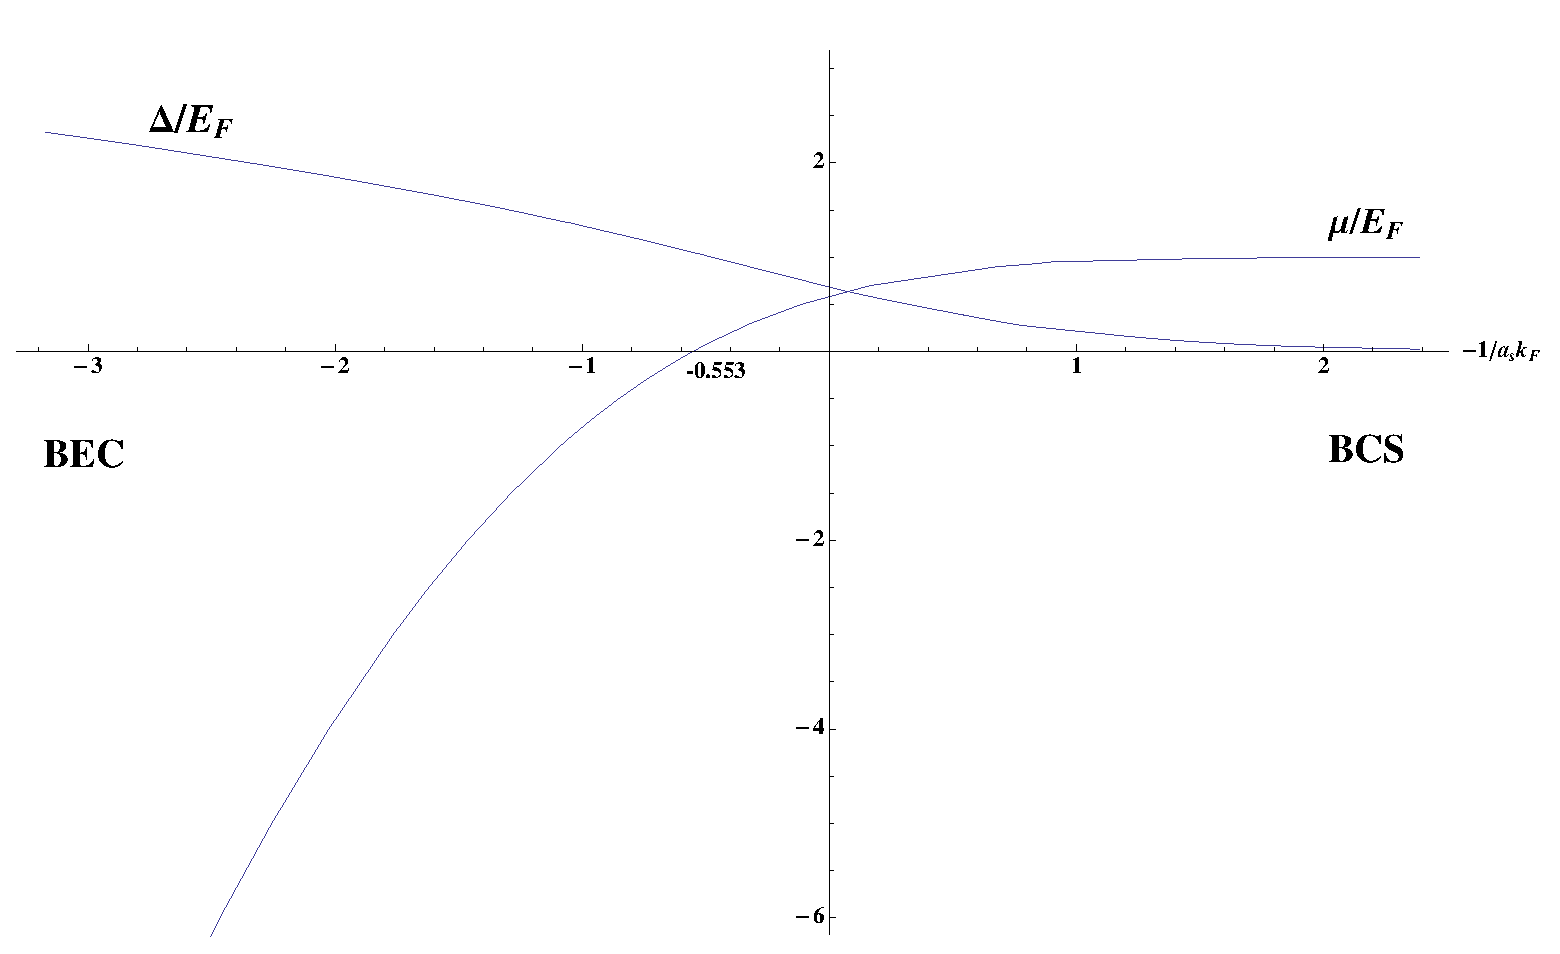
\includegraphics[width=0.8\textwidth]{SingleChannelCrossoverMuDelta}
\caption{The chemical potential $\mu$ and gap $\Delta$ in the mean field level over crossover} 
\label{fig:pathInt:meanField}
{\small All quantities in the unit of energy ($\mu$, $\Delta$) are rescaled with the Fermi energy $E_{F}$ and the s-wave scattering length $a_{s}$ is rescaled with $1/k_{F}$.  }
\end{center}
\end{figure}



\section{Gaussian fluctuation and collective modes}\label{sec:collective1}
We can expand the partition function Eq. (\ref{eq:pathInt:DeltaPF}) around the mean-field value, $\Delta(\vr,\tau)=\Delta_{0}+\theta(\vr,\tau)$. The linear order of the  expansion is zero because $\Delta_{0}$ is the saddle point.  The next order gives us the bilinear terms on $\theta$, i.e., correlation of bosonic fields $\Delta$ (four-fermion correlation).  Note that here the Hamiltonian only has a contact-type potential, therefore it cannot cover the situation of a charged system where long-range Columnb interaction cannot be neglected.  We limit ourselves to the neutual case.  Nevertheless, it is conceivable that a more realistic short-range potential only renormalizes some parameters in the following calculation while leaves the qualitative result unmodified.  

Notice that we can expand the second term in Eq. (\ref{eq:pathInt:DeltaPF}) for $\hat{G}{}^{-1}=\hat{G}_{0}^{-1}+\hat{K}$
\begin{equation}\label{eq:pathInt:expand}
\tr\ln \hat{G}^{-1}=\tr\ln\hat{G_{0}}^{-1}+\tr(\hat{G_{0}}\hat{K})-\nth{2}\tr(\hat{G_{0}}\hat{K}\hat{G_{0}}\hat{K})+\cdots
\end{equation}
In our case,
\begin{equation}
\hat{K}=\begin{pmatrix}
0&\theta\\
\theta^{*}&0
\end{pmatrix}
\end{equation}
Here the linear terms of $\hat{K}$ or $\theta$ ($\theta^{*}$) are zero as the saddle point condition.  To the second order, the action is 
\begin{equation}\label{eq:pathInt:DeltaActionGaussian}
S[\Delta_{0},\theta,\theta^{*}]=S[\Delta_{0}]+
	\nth{2g}\tr(\hat{K}\hat{K})+\nth{2}\tr(\hat{G_{0}}\hat{K}\hat{G_{0}}\hat{K})
\end{equation}
Write the last term into the momentum representation
\begin{equation}
\tr(\hat{G_{0}}\hat{K}\hat{G_{0}}\hat{K})=\sum_{q,p}\Tr\br{G_{0}({p})K_{q}G_{0}{}({p-q})K_{-q}}
\end{equation}
Notice that the second ``$\Tr$'' and following ``$\Tr$'' in this section only runs in Nambu spinor space and $q={(\vq,q_{l})}$, $p=(\vp,p_{n})$ are all four momentum, where $q_{l}$ is the bosonic Matsubara frequency while $p_{n}$ is the fermionic Matsubara frequency.
\begin{equation}
K_{p_{0},p_{0}+q}=K_{q}=\begin{pmatrix}
0&\theta_{q}\\
\theta^{*}_{-q}&0
\end{pmatrix}
\end{equation}
And we remember that $G_{0}(p)=G_{0}{}_{p,p}$
If we introduce  a new vector 
\begin{equation}
\theta{(q)}=\begin{pmatrix}\theta_{q}\\\theta^{*}_{-q}\end{pmatrix}\qquad
\theta^{\dg}{(q)}=\begin{pmatrix}\theta^{*}_{q}&\theta_{-q}\end{pmatrix}
\end{equation}
the action can be rewritten into a more compact form
\begin{equation}
S[\Delta_{0},\theta,\theta^{*}]=S[\Delta_{0}]+\nth{2}\sum_{q}\mbr{\theta^{\dg}(q)\mathbf{M}(q)\theta(q)}
\end{equation}
Notice that we can always choose a real $\Delta_{0}$ and therefore $G_{0}{\ _{12}}(p)=G_{0}{\ _{21}}(p)$, we have 
\begin{equation}
\mathbf{M}_{q,q}=\mathbf{M}(q)=
\begin{pmatrix}
\nth{g}+\sum_{p}G_{0}{\ }_{11}(p)G_{0}{\ }_{22}(p-q)&\sum_{p}G_{0}{\ }_{12}(p)G_{0}{\ }_{12}(p-q)\\
\sum_{p}G_{0}{\ }_{12}(p)G_{0}{\ }_{12}(p-q)&\nth{g}+\sum_{p}G_{0}{\ }_{11}(p-q)G_{0}{\ }_{22}(p)
\end{pmatrix}
\end{equation}
The summation over  the (fermionic) Matsubara frequency of $p_{n}$ can be carried out at zero temperature

\begin{equation}
\begin{split}
M_{11}(q)&=M_{22}(-q)\\
	&=\nth{g}+\sum_{\vp{,}p_{n}}G_{0}{\ }_{11}(p)G_{0}{\ }_{22}(p-q)\\
	&=\nth{g}+\sum_{\vp}\br{\frac{u^{2}u'^{2}}{iq_{l}-E-E'}-\frac{v^{2}v'^{2}}{iq_{l}+E+E'}}
\end{split}
\end{equation}
\begin{equation}
\begin{split}
M_{12}(q)&=M_{21}(q)\\
	&=\sum_{\vp{,}p_{n}}G_{0}{\ }_{12}(p)G_{0}{\ }_{12}(p-q)\\
	&=\sum_{\vp}uvu'v'\br{\nth{iq_{l}+E+E'}-\nth{iq_{l}-E-E'}}
\end{split}
\end{equation}
where $u=u_{\vp}$, $v=v_{\vp}$, $E=E_{\vp}$ and $u'=u_{\vp-\vq}$, $v'=v_{\vk-\vq}$, $E'=E_{\vk-\vq}$.  $u_{\vk}$, $v_{\vk}$, $E_{\vk}$ are as defined usually in BCS literature. 
\begin{equation}
v_{\vk}^{2}=1-u_{\vk}^{2}=\nth{2}\br{1-\frac{\xi_{\vk}}{E_{\vk}}}
\end{equation}
 The $G^{(M)}=\mathbf{M}^{-1}$ is the correlation function of $\theta$ (or $\Delta$) and its poles give the spectrum of collective modes as every  $\theta_{q}$ (or $\Delta_{q}$) involves many fermions moving in a coherent manner.  So the spectrum of collective modes can be determined by finding poles of $G^{(M)}$, $\det{M(\omega,\vq)}=0$ after we analytically continue for the frequency $iq_{l}\rightarrow\omega+i0^{+}$.  
 
For low energy modes, where $\omega,\,\abs{\vq}^{2}$ both are much smaller than $\min\bbr{E_{\vk}}=\Delta_{0}$ (or $\sqrt{\mu^{2}+\Delta^{2}}$ for $\mu<0$), we can expand $M$ with $\omega$ and $\vq$.  The lowest order has the form $\omega\approx{}c\,q$, which suggests a sound wave as expected for any Goldstone mode.  At BCS side, $c=v_{F}/\sqrt{3}$, where $v_{F}$ is Fermi velocity.  This coincides with the famous Anderson-Bogoliubov mode.  At the BEC side, we get $c^{2}=\Delta^{2}/8m\abs{\mu}=v_{F}^{2}(k_{F}a_{s})/3\pi=4\pi{}n_{B}a_{B}/m_{B}$, which fits the low momentum part of Bogoliubov spectrum of bosons gas.  Here $m_{B}=2m$ is the molecule mass, $n_{B}=n/2$ is the molecule density and $a_{B}=2a_{s}$ is the inferred  interaction between molecules.  This value differs from the result of more accurate calculation from the few-body theory, $a_{B}=0.6a_{s}$ \cite{Petrov}, which indicates the possible deficiency of the current theory. 


\section{An alternative method to invert the Green's function\label{sec:diagonalizeGreen1}}
In the above section, we inverted the  Gor'kov green function matrix Eqs. (\ref{eq:pathInt:nG}, \ref{eq:pathInt:G0}) directly and it is not hard to do as a $2\times2$ matrix in the  momentum space.   Alternatively, we can use a different approach which proves to be more convenient in the two-channel problem.  First, we diagonalize $\nG$ with a unitary transformation $T$, in the momentum space
\begin{equation}
\nG=\mtrx{i\omega_{n}-\xi_{k}&\Delta\\\bar\Delta&i\omega_{n}+\xi_{k}}=T^{\dg}BT
\end{equation}
It is easy to show that such $T$ and $B$ satisfying above equation are
\begin{equation}
T=\mtrx{u_{k}&v_{k}\\-v_{k}^{*}&u_{k}}\qquad{}B=\mtrx{i\omega_{n}+E_{k}&0\\0&i\omega_{n}-E_{k}}
\end{equation}
where $u_{k}^{2}(v_{k}^{2})=\nth{2}(1\pm\xi_{k}/E_{k})$ and $E_{k}=\sqrt{\xi^{2}_{\vk}+\Delta^{2}}$ are conventionally defined quantities in the BCS theory.   Actually, this transformation is nothing but the Bogoliubov canonical transformation, and the $B$ matrix simply describes the spectrum of the fermionic quasi-particles.  Now it is easy to invert $\nG$
\begin{equation}
\mathcal{G}=T^{\dg}B^{-1}T
\end{equation}
Green's function $\mathcal{G}$ takes a more conventional form $A/(i\omega_{n}\pm{}E_{k})$ without any dependency on frequency in nominator as Eq. (\ref{eq:pathInt:G0}). Matsubara frequency summation over $G_{0}(k)$ in the mean-field and $G_{0}(k)G_{0}(k+q)$ in the Gaussian order are then easier to perform  as in text-book.  
